\title{Study Guide for Final Exam for Algebra-Based Physics-2: Electricity, Magnetism, and Modern Physics (PHYS135B-01)}
\author{Dr. Jordan Hanson - Whittier College Dept. of Physics and Astronomy}
\date{\today}
\documentclass[10pt]{article}
\usepackage[a4paper, total={18cm, 27cm}]{geometry}
\usepackage{outlines}
\usepackage[sfdefault]{FiraSans}
\usepackage{hyperref}
\usepackage{graphicx}
\begin{document}
\maketitle

\begin{enumerate}
\item \textbf{Electric charge and electric fields}
\begin{enumerate}
\begin{figure}[ht]
\centering
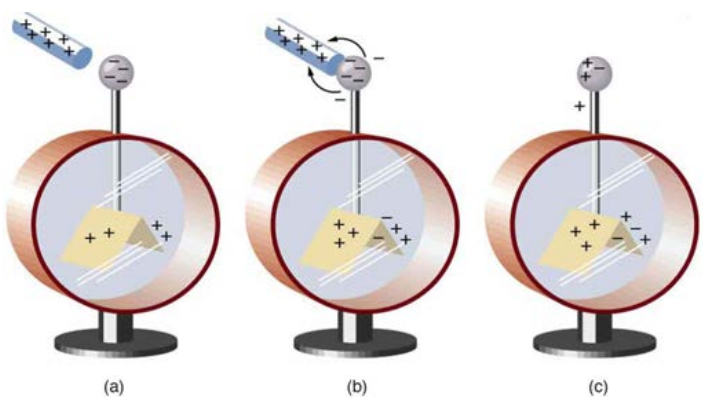
\includegraphics[width=0.35\textwidth]{figures/elec.png}
\caption{\label{fig:elec} Touching charge to an electroscope.  A glass rod with a positive net charge is moved near the ball.  Initially, the electroscope is electrically neutral.}
\end{figure}
\item Which of the following is true of the electroscope in part (a) of Fig. \ref{fig:elec}?
\begin{itemize}
\item A: The net charge in the gold leaves plus the ball is positive.
\item B: The net charge in the gold leaves plus the ball is negative.
\item C: The net charge in the gold leaves plus the ball is zero.
\item D: The net charge in the gold leaves plus the ball is equal and opposite to that of the rod.
\end{itemize}
\item Which of the following is true of the electroscope in part (b) of Fig. \ref{fig:elec}?
\begin{itemize}
\item A: Touching the positive rod to the ball causes current to flow.
\item B: Touching the positive rod to the ball leaves the electroscope with a positive charge.
\item C: Touching the positive rod to the ball increases the net charge of the rod.
\item D: A and B
\end{itemize}
\item Which of the following is true of the electroscope in part (c) of Fig. \ref{fig:elec}?
\begin{itemize}
\item A: Charge redistributes evenly, and the leaves remain apart.
\item B: Charge redistributes evenly, and the leaves close.
\item C: Charge redistributes non-uniformly and so the leaves remain apart.
\item D: Charge redistributes non-uniformly and so the leaves close.
\end{itemize}
\begin{figure}[hb]
\centering
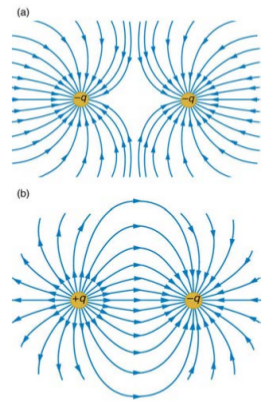
\includegraphics[width=0.2\textwidth]{figures/dipole.png}
\caption{\label{fig:dipole} (Top) The electric field of two positive charges. (Bottom) The electric field of a dipole.}
\end{figure}
\item A test charge $+q$ in between the charges in Fig. \ref{fig:dipole} (a) will:
\begin{itemize}
\item A: Move to the left
\item B: Move to the right
\item C: Remain stationary
\item D: Move down
\end{itemize}
\item A test charge $+q$ in between the charges in Fig. \ref{fig:dipole} (b) will:
\begin{itemize}
\item A: Move to the left
\item B: Move to the right
\item C: Remain stationary
\item D: Move down
\end{itemize}
\item If a uniform external electric field points up in Fig. \ref{fig:dipole} (a), the charges will
\begin{itemize}
\item A: Move to the left
\item B: Move to the right
\item C: Remain stationary
\item D: Move up
\end{itemize}
\item If a uniform external electric field points up in Fig. \ref{fig:dipole} (b), the dipole will
\begin{itemize}
\item A: Rotate clockwise
\item B: Rotate counter-clockwise
\item C: Remain stationary
\item D: Move down
\end{itemize}
\end{enumerate}
\item \textbf{Electric potential and electric fields}
\begin{figure}[hb]
\centering
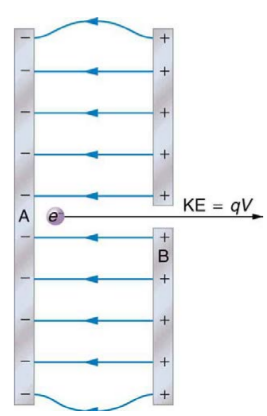
\includegraphics[width=0.2\textwidth]{figures/plate2.png}
\caption{\label{fig:plate2} An electron is accelerated through a potential $V$.}
\end{figure}
\begin{enumerate}
\item Suppose the voltage in Fig. \ref{fig:plate2} is 1 kV.  The final energy of the electron is
\begin{itemize}
\item A: 1 Joule
\item B: 1 eV
\item C: 1 keV
\item D: 10 Joules
\end{itemize}
\item Suppose the voltage in Fig. \ref{fig:plate2} is doubled.  The final velocity
\begin{itemize}
\item A: Increases by a factor of 2
\item B: Increases by a factor of $\sqrt{2}$
\item C: Increases by a factor of 4
\item D: Decreases by a factor of 2
\end{itemize}
\item Recall that the relationship between the voltage, electric field, and separation in a capacitor is $V = E d$.  What is the electric field inside a capacitor with separation $0.1$ mm, and is charged at $12$ V?
\begin{itemize}
\item A: 1.2 V/m
\item B: 1.2 mV/m
\item C: 120 kV/m
\item D: 120 V/m
\end{itemize}
\item Draw a graph of the voltage versus separation for the capacitor in the previous problem.  Label which side of the graph corresponds to positive charge and which side corresponds to negative charge.  Label the axes with approprate units. \\ \vspace{3cm}
\item Recall that the definition of capacitance is $Q = CV$, for a charge $Q$ and voltage $V$.  How much charge is stored on the capacitor in the previous two problems ($V = 12$ V), if the capacitance is $1 \mu$F? \\ \vspace{2cm}
\item The capacitance of a parallel plate capacitor is $C = \epsilon_0 A/d$, where $A$ is the area of the plates, $d$ is the separation between the plates, and $\epsilon_0 = 8.85 \times 10^{-12}$ N$^{-1}$ C$^2$ m$^{-2}$.  What is the capacitance of a capacitor with an area of 4 mm$^2$ and a separation of 1 mm? \\ \vspace{2cm}
\item If two such capacitors are connected \textit{in parallel}, what is the total capacitance?  What is the total capacitance if they are connected \textit{in series}? \\ \vspace{2cm}
\end{enumerate}
\item \textbf{Electric current, resistance, and Ohm's law}
\begin{enumerate}
\item Recall that Ohm's law states that $V = iR$, and that resistors in series add, while resistors in parallel add in reciprocal.  Find the total current from the battery in the circuit drawn in Fig. \ref{fig:circuit}.
\begin{figure}[hb]
\centering
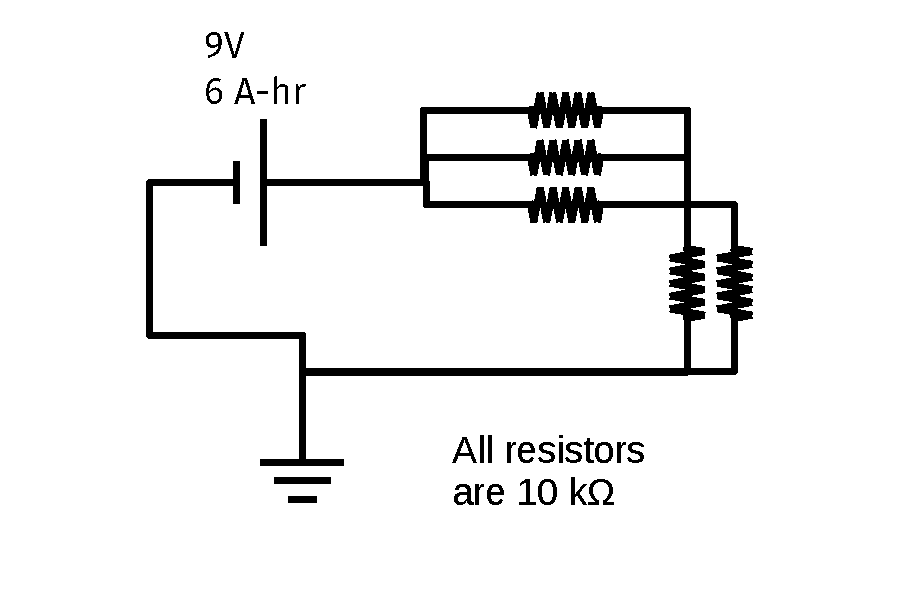
\includegraphics[width=0.5\textwidth]{figures/circuitExample1.pdf}
\caption{\label{fig:circuit} A DC circuit with a battery voltage of 9V and five identical resistors.}
\end{figure}
\item How long before the charge in the battery is drained in the circuit in Fig. \ref{fig:circuit}?
\begin{figure}
\centering
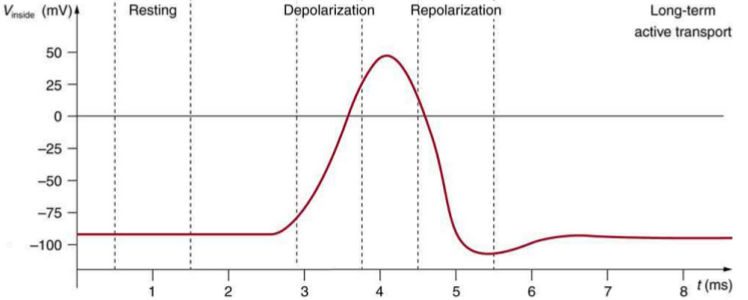
\includegraphics[width=0.5\textwidth]{figures/action.png}
\caption{\label{fig:action} The voltage versus time of a nerve action pulse.}
\end{figure}
\item How are the four stages of the voltage pulse above created in the human body? \\ \vspace{3cm}
\end{enumerate}
\item \textbf{•}
\end{enumerate}
\end{document}